\documentclass[journal,12pt,twocolumn]{IEEEtran}

\usepackage{setspace}
\usepackage{gensymb}
\singlespacing
\usepackage[cmex10]{amsmath}

\usepackage{amsthm}

\usepackage{mathrsfs}
\usepackage{txfonts}
\usepackage{stfloats}
\usepackage{bm}
\usepackage{cite}
\usepackage{cases}
\usepackage{subfig}

\usepackage{longtable}
\usepackage{multirow}

\usepackage{enumitem}
\usepackage{mathtools}
\usepackage{steinmetz}
\usepackage{tikz}
\usepackage{circuitikz}
\usepackage{verbatim}
\usepackage{tfrupee}
\usepackage[breaklinks=true]{hyperref}
\usepackage{graphicx}
\usepackage{tkz-euclide}

\usetikzlibrary{calc,math}
\usepackage{listings}
    \usepackage{color}                                            %%
    \usepackage{array}                                            %%
    \usepackage{longtable}                                        %%
    \usepackage{calc}                                             %%
    \usepackage{multirow}                                         %%
    \usepackage{hhline}                                           %%
    \usepackage{ifthen}                                           %%
    \usepackage{lscape}     
\usepackage{multicol}
\usepackage{chngcntr}

\DeclareMathOperator*{\Res}{Res}
\newtheorem{theorem}{Theorem}[section]
\newtheorem{corollary}{Corollary}[theorem]
\newtheorem{lemma}[theorem]{Lemma}
\newtheorem{definition}{Definition}[section]
\renewcommand\thesection{\arabic{section}}
\renewcommand\thesubsection{\thesection.\arabic{subsection}}
\renewcommand\thesubsubsection{\thesubsection.\arabic{subsubsection}}

\renewcommand\thesectiondis{\arabic{section}}
\renewcommand\thesubsectiondis{\thesectiondis.\arabic{subsection}}
\renewcommand\thesubsubsectiondis{\thesubsectiondis.\arabic{subsubsection}}


\hyphenation{op-tical net-works semi-conduc-tor}
\def\inputGnumericTable{}                                 %%

\lstset{
%language=C,
frame=single, 
breaklines=true,
columns=fullflexible
}
\begin{document}

\newcommand{\BEQA}{\begin{eqnarray}}
\newcommand{\EEQA}{\end{eqnarray}}
\newcommand{\define}{\stackrel{\triangle}{=}}
\bibliographystyle{IEEEtran}
\raggedbottom
\setlength{\parindent}{0pt}
\providecommand{\mbf}{\mathbf}
\providecommand{\pr}[1]{\ensuremath{\Pr\left(#1\right)}}
\providecommand{\qfunc}[1]{\ensuremath{Q\left(#1\right)}}
\providecommand{\sbrak}[1]{\ensuremath{{}\left[#1\right]}}
\providecommand{\lsbrak}[1]{\ensuremath{{}\left[#1\right.}}
\providecommand{\rsbrak}[1]{\ensuremath{{}\left.#1\right]}}
\providecommand{\brak}[1]{\ensuremath{\left(#1\right)}}
\providecommand{\lbrak}[1]{\ensuremath{\left(#1\right.}}
\providecommand{\rbrak}[1]{\ensuremath{\left.#1\right)}}
\providecommand{\cbrak}[1]{\ensuremath{\left\{#1\right\}}}
\providecommand{\lcbrak}[1]{\ensuremath{\left\{#1\right.}}
\providecommand{\rcbrak}[1]{\ensuremath{\left.#1\right\}}}
\theoremstyle{remark}
\newtheorem{rem}{Remark}
\newtheorem*{remark}{Remark}
\newcommand{\sgn}{\mathop{\mathrm{sgn}}}
\providecommand{\abs}[1]{\vert#1\vert}
\providecommand{\res}[1]{\Res\displaylimits_{#1}} 
\providecommand{\norm}[1]{\lVert#1\rVert}
%\providecommand{\norm}[1]{\lVert#1\rVert}
\providecommand{\mtx}[1]{\mathbf{#1}}
\providecommand{\mean}[1]{E[ #1 ]}
\providecommand{\fourier}{\overset{\mathcal{F}}{ \rightleftharpoons}}
%\providecommand{\hilbert}{\overset{\mathcal{H}}{ \rightleftharpoons}}
\providecommand{\system}{\overset{\mathcal{H}}{ \longleftrightarrow}}
	%\newcommand{\solution}[2]{\textbf{Solution:}{#1}}
\newcommand{\solution}{\noindent \textbf{Solution: }}
\newcommand{\cosec}{\,\text{cosec}\,}
\providecommand{\dec}[2]{\ensuremath{\overset{#1}{\underset{#2}{\gtrless}}}}
\newcommand{\myvec}[1]{\ensuremath{\begin{pmatrix}#1\end{pmatrix}}}
\newcommand{\mydet}[1]{\ensuremath{\begin{vmatrix}#1\end{vmatrix}}}
\numberwithin{equation}{subsection}
\makeatletter
\@addtoreset{figure}{problem}
\makeatother
\let\StandardTheFigure\thefigure
\let\vec\mathbf
\renewcommand{\thefigure}{\theproblem}
\def\putbox#1#2#3{\makebox[0in][l]{\makebox[#1][l]{}\raisebox{\baselineskip}[0in][0in]{\raisebox{#2}[0in][0in]{#3}}}}
     \def\rightbox#1{\makebox[0in][r]{#1}}
     \def\centbox#1{\makebox[0in]{#1}}
     \def\topbox#1{\raisebox{-\baselineskip}[0in][0in]{#1}}
     \def\midbox#1{\raisebox{-0.5\baselineskip}[0in][0in]{#1}}
\vspace{3cm}
\title{Assignment 5}
\author{Yashas Tadikamalla - AI20BTECH11027}
\maketitle
\newpage
\bigskip
\renewcommand{\thefigure}{\theenumi}
\renewcommand{\thetable}{\theenumi}
Download all python codes from 
\begin{lstlisting}
https://github.com/YashasTadikamalla/EE3900/blob/main/Assignment5/codes
\end{lstlisting}
%
and latex-tikz codes from 
%
\begin{lstlisting}
https://github.com/YashasTadikamalla/EE3900/blob/main/Assignment5/Assignment5.tex
\end{lstlisting}
\section{Problem (Quadratic Forms Q2.31)}
Find the equation of hyperbola with focii \myvec{0\\\pm12} and length of latus rectum 36.
\section{Solution}
\begin{theorem}
The equation of  a conic with directrix $\vec{n}^{\top}\vec{x} = c$, eccentricity $e$ and focus $\vec{F}$ is given by 
\begin{align}
    \label{eq:conic_quad_form}
    \vec{x}^{\top}\vec{V}\vec{x}+2\vec{u}^{\top}\vec{x}+f=0
    \end{align}
where     
\begin{align}
\label{eq:conic_quad_form_v}
\vec{V} &=\norm{\vec{n}}^2\vec{I}-e^2\vec{n}\vec{n}^{\top}, \\
\label{eq:conic_quad_form_u}
\vec{u} &= ce^2\vec{n}-\norm{\vec{n}}^2\vec{F}, \\
\label{eq:conic_quad_form_f}
f &= \norm{\vec{n}}^2\norm{\vec{F}}^2-c^2e^2
\end{align}
\end{theorem}
\begin{theorem}
The eccentricity of the conic represented by \eqref{eq:conic_quad_form} is given by
\begin{align}
e= \sqrt{1-\frac{\lambda_1}{\lambda_2}}
\label{eq:e}
\end{align}
\end{theorem}
\begin{theorem}
If \eqref{eq:conic_quad_form} represents a hyperbola, the lengths of the semi-major and semi-minor axes are given by
\begin{align}
\sqrt{\frac{\vec{u}^{\top}\vec{V}^{-1}\vec{u} -f}{\lambda_1}}, 
       \sqrt{\frac{f-\vec{u}^{\top}\vec{V}^{-1}\vec{u}}{\lambda_2}}
       \label{eq:ab}
\end{align}
respectively, where $\lambda_1>0,\lambda_2<0$
\end{theorem}
Given, length of latus rectum is 36 and
\begin{align}
    \vec{F} =\myvec{0\\ 12}\Rightarrow\norm{\vec{F}}=12
\end{align}
Let $\vec{u}^{\top}\vec{V}^{-1}\vec{u}-f=\alpha$. From \eqref{eq:ab},\eqref{eq:e} 
\begin{align}
    \sqrt{\frac{\alpha}{\lambda_1}}\sqrt{1-\frac{\lambda_1}{\lambda_2}}=12\label{eq:one}\\
    \dfrac{2\brak{\dfrac{-\alpha}{\lambda_2}}}{\sqrt{\dfrac{\alpha}{\lambda_1}}}=36\label{eq:two}
\end{align}
Dividing \eqref{eq:one} by \eqref{eq:two} gives
\begin{align}
    \dfrac{\lambda_1}{\lambda_2}&=-3\\
    \Rightarrow e&=2\\
    \Rightarrow \sqrt{\frac{\alpha}{\lambda_1}}&=6
\end{align}
The directrix of this hyperbola passes through the point $\myvec{0\\3}$ and is perpendicular to the y-axis. 
\begin{align}
    \myvec{0&1}\brak{\vec{x}-\myvec{0\\3}} = 0\\
    \implies \myvec{0&1}\vec{x} = 3
\end{align}
Comparing it with $\vec{n}^{\top}\vec{x} = c$
\begin{align}
    \vec{n} = \myvec{0\\1}, c = 3\Rightarrow \norm{\vec{n}} = 1
\end{align}
Calculating $\vec{V}, \vec{u}$ and $f$,
\begin{align}
    \vec{V}&=1^2\myvec{1&0\\0&1} - 2^2\myvec{0\\1}\myvec{0&1}\\
    &=\myvec{1&0\\0&1}-\myvec{0&0\\0&4}=\myvec{1&0\\0&-3}\\
    \vec{u}&= 3(2^2)\myvec{0\\1} - 1^2\myvec{0\\12}=\myvec{0\\0}\\
    f &= 1^2(12^2) - 3^2(2^2)= 108
\end{align}
Hence, the required equation is
\begin{align}
    \vec{x}^{\top}\myvec{1&0\\0&-3}\vec{x}+108=0
\end{align}
\begin{figure}[!h]
 \centering
 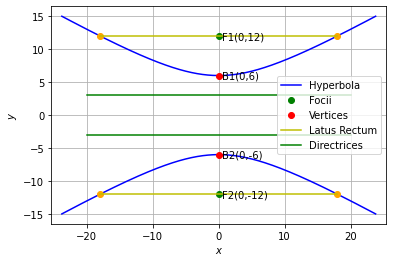
\includegraphics[width=\columnwidth]{Assignment5.png}
 \caption{Hyperbola}
 \label{plot}
\end{figure}
\end{document}